\chapter{Related Work}
\label{chap:relatedwork}

This chapter covers work related to parking space sensing and machine learning. Section \ref{sec:parksensing} discusses different technologies and approaches to sensing current parking situations in cities. Furthermore, a comparison is provided that results in a discussion of advantages and disadvantages of the specific approaches. In Section \ref{sec:acquiring_parking_space_maps}, the need for parking space maps will be discussed as well as how they can be obtained using several sensing vehicles.



\section{Approaches to Parking Space Sensing}
\label{sec:parksensing}

There already exist numerous approaches for detecting the states of parking spaces as well as the parking situation in a city. In this section, parking detection approaches are categorized in six different categories and representatives of each category are discussed. The six categories (shown in Figure \ref{fig:parking_space_sensing_methods}) are stationary parking space sensing with dedicated sensors (Section \ref{sec:stationary_park_sensing}), parking space sensing using stationary cameras (Section \ref{sec:stationary_park_sensing_cameras}), counting in- and outgoing vehicles (Section \ref{sec:counting_in_out_park_sensing}), event detection based parking space sensing (Section \ref{sec:event_detection_park_sensing}), and drive-by parking space sensing using either a camera (Section \ref{sec:related_driveby_park_sensing_cameras}) or a distance sensor (\ref{sec:related_driveby_park_sensing_distance}). After all detection strategies have been discussed an overall comparison is presented in Section \ref{sec:comparison_park_sensing_approaches}.

\begin{figure}
	\centering
	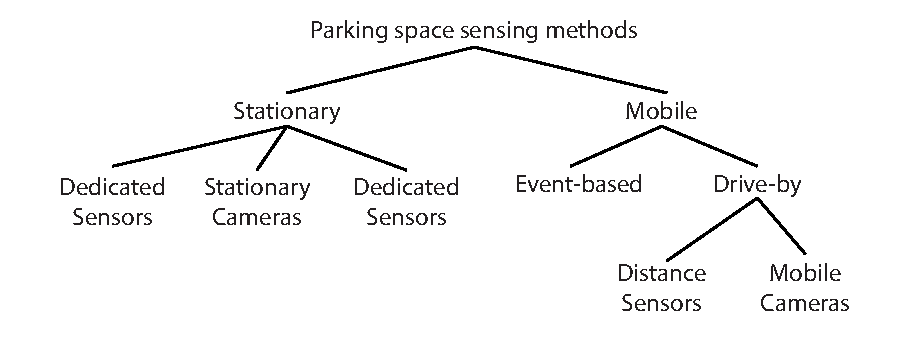
\includegraphics[width=0.75\textwidth]{img/parking_space_sensing_methods.eps}
	\caption{Overview of all discussed parking space sensing approaches.}
	\label{fig:parking_space_sensing_methods}
\end{figure}

\subsection{Stationary Parking Space Sensing with Dedicated Sensors}
\label{sec:stationary_park_sensing}

The most obvious and technically simple solution to parking space sensing is to use stationary sensors to determine the state of parking spaces. Usually one sensor per parking space is used which determines its state (occupied or vacant) and sends this state to a central server. Several reference projects already exist implementing this technique\cite{SFPark, VehicleSense}. In this section, as a representation of all the similar systems, the SFpark project will be examined.

In San Francisco a first prototype of the SFpark project \cite{SFPark} has been employed from 2008 to 2011. Wireless stationary sensors have been placed at about 8.200 road side parking spaces in specific down town areas in San Francisco with high amounts of traffic. These sensors detect the state of one parking space in real-time and send this information to a central server. Furthermore, parking lots also count the in- and outgoing vehicles and share this information, so that the parking situation in the areas with parking space sensing can be derived. The gained information is shared as open data. Third party developers and researchers can also use the dataset for all kind of projects and purposes. Furthermore, there exists an app from SFpark itself to help drivers find available parking spaces nearby, navigate to them, and pay as they go with their phones.

A top priority goal of the SFpark project is to increase the availability of parking spaces in every block throughout the city. To achieve this goal, they are using demand responsive pricing. If (almost) all parking spaces in a neighbourhood are occupied for a long time, they raise the price in this specific area. If no parking spaces are occupied they lower prices. This leads to high overall parking space availabilities (20 - 40\%) and also to lower traffic congestion and lower greenhouse gas emissions. However, besides the advantages of high accuracy and being a real-time system, there also are disadvantages. First of all, only metered parking spaces can be tracked, as sensors have to be installed per parking space. Thus, areas where parking is allowed but there are no clearly marked parking spaces cannot be sensed with a reasonable accuracy. Another drawback are the high overall costs. The about 8.200 stationary sensors have to be bought, installed and maintained, which obviously causes high costs while only covering a tiny fraction of the overall San Francisco down town. So if the system should be available in the whole city, costs would increase dramatically.





\subsection{Stationary Parking Space Sensing using Cameras}
\label{sec:stationary_park_sensing_cameras}

Another approach while using stationary sensors is to use fixed deployed cameras which continuously record images of parking areas and analyze them for vacant parking spaces. Cameras can monitor up to one hundred parking spaces simultaneously with an accuracy of up to 96\% \cite{DiMauro2016}. Challenges of image detection are different lightning and weather conditions as well as occlusions depending on the angle the camera records the parking scene. Detection algorithms may use standard digital image processing as well as deep learning and convolutional neural networks (CNNs) as discussed in the following.


\paragraph{Parking detection using digital image processing}

There exist a few common approaches using digital image processing to detect the state of parking spaces using a captured image of a parking area. First of all, edge detection is often used for parking space classification. Common edge detectors such as the Canny Edge Detector \cite{Canny1986} or the Sobel Operator \cite{Sobel} can be used to derive the edge pixels of an image. The edges or edge pixels are counted and if the amount is above a certain threshold, the space will be detected as occupied. The assumption behind this approach is, that usually a vacant parking space has a plain surface and therefore a low amount of edges whereas an image of a parking car should have a lot of edges. Blumer et al. \cite{Blumer2012} and Liu et al. \cite{stationary_camera_sensing} both use this technique as part of their algorithms.

A slightly different yet related approach is object counting \cite{stationary_camera_sensing}. The edges of the image segment of a parking space are analyzed and closed contours (treated as objects) are detected and counted. Then, depending on a threshold which has to be set first, a parking space is classified as either vacant or occupied depending on the object count.

Another common image processing technique leverages foreground- and background information of the images. Here, the main background color is identified and compared to the whole image. The background of a parking space can either be defined via extracting a certain part of the image, which should always represent the main background color of a parking space's pavement (done by Blumer et al. \cite{Blumer2012}), or by using the color which is most present in the image assuming that the background uses the most pixels in the recorded image (done by Liu et al. \cite{stationary_camera_sensing}). After the background color is identified it is subtracted from the original image. Using thresholding, foreground and background pixels are identified and counted. Depending on the count of the respective pixels, the parking space is then classified as vacant or occupied.

Liu et al. \cite{stationary_camera_sensing} use all of the above mentioned techniques in combination to build a stable prototype. They only test their prototype indoors which is why weather and lightning conditions do not cause problems. With sensing only a maximum of seven cars, it provids an ensemble technique, leveraging the approaches from \cite{Blumer2012} and \cite{stationary_camera_sensing} in conjunction, which should lead to a more reliable system. However, the work does not include an evaluation of how well their algorithm performed on a larger dataset. Another ensemble method is developed by Blumer et al \cite{Blumer2012}. They use edge counts and background/foreground information as input for different machine learning techniques, which then classify a parking space as vacant or occupied. The plain algorithm achieves an accuracy of about 77.8\%. By improving the algorithm using frames of preceding and following images to identify parking/unparking events, an accuracy of about 88.8\% is achieved.



\paragraph{Parking image processing using deep learning and CNNs}

In recent years deep learning gained a lot of attention in the field of machine learning. Deep learning is a specific variant of neural networks with a high amount of hidden layers. For example in image recognition, convolutional neural networks (CNNs) nowadays perform as well as humans in classifying everyday objects in digital images. A CNN is a neural network with a possibly large amount of hidden layers of which some of them are convolutional layers. In the case of image recognition, CNNs take the spatial relationships between neighbouring pixels into account. This rise in learning power also leads to projects which try to train CNNs in classifying parking situations while using camera images of a parking area.

Amato et al. \cite{Amato2016} train two different CNNs on classifying parking space states and compare their performances afterwards. They use the publicly available PKLot dataset as well as a dataset collected by themselves to train and evaluate the neural networks. In total over 700.000 images in different weather conditions and with different levels of quality are processed (in some situations parking lots are almost fully occluded by trees or lamp posts, etc.). The results of the CNN's classifications are promising. Despite the fact that some of the images do not exactly match the parking space and there are a lot of occlusions, the best performing deep neural network achieves an accuracy of above 91\% on all subsets of the datasets.

Another work in the field of deep learning is described by Di Mauro \cite{DiMauro2016}. They also use CNNs and the PKLot dataset, as well as a self-acquired dataset. However, a slightly different CNN is employed together with pseudo-labelling of the data, which can be seen as semi-supervised approach. When using pseudo-labelling both labelled and unlabelled data are used at the same time to train the network. For unlabelled data, the label which was computed by the CNN in the forward pass is used. Therefore, the method is termed pseudo-labelling. Furthermore, a different loss function is used as the pseudo-labelled data has much less significance than the ground truth labelled data. Di Mauro et al. train the CNN with about 5\% of the data and achieve an accuracy of above 96\% with a the fully supervised approach. The pseudo-labelling approach reaches about the same level of accuracy, however, the dataset has to be balanced for it to work properly.


\paragraph{Advantages and disadvantages of using stationary cameras}

Advantages of cameras are the high level of accuracy they reach while covering a lot of cars at once. However, for all of the above discussed approaches to work, cameras would have to be calibrated manually before their usage to know where parking spaces are located. Furthermore, most of the research focuses on the use of cameras for detecting the parking space situation of a single parking lot with many cars and not for road side parking spaces. For road side parking space detection to work at a city wide scope, cameras would have to be mounted at least at every block. Similar to the dedicated sensors per parking space (Section \ref{sec:stationary_park_sensing}), this would cause high costs not only with respect to hardware but also due to installation and maintenance expenses. Furthermore, mounting cameras throughout the city obviously also brings up privacy issues.





\subsection{Counting In- and Outgoing Vehicles}
\label{sec:counting_in_out_park_sensing}

A rather simple approach of estimating the number of free parking spaces is to count in- and outgoing vehicles at parking zones. Zadeh et al. \cite{smarturbanparkingdetection} present a prototype which counts all in- and outgoing vehicles using a Raspberry Pi and two ultrasonic range finders at each gate. Ultrasonic sensors measure the distance from the side of the road to a potentially passing vehicle. Two ultrasonic sensors in sequence are needed. According to the order in which the ultrasonic sensors detect a passing vehicle it is decided whether a vehicle is going in or out. Furthermore,
the two sensors are also used to differentiate a passing person from a vehicle. Both sensors are as far apart as they can detect a vehicle at the same time but not a person. This way, misleading detections of passengers are filtered.

This approach is technically simple to implement and the hardware costs are also very low. However, this system is only designed for parking lots which have a low number of gates where cars go in and out and not for a city wide deployment. For closed parking areas it is easy to detect in- and outgoing vehicles whereas it is hard to do so in open traffic and street scenarios. Furthermore, the counting also will not work with ultrasonic sensors in open street scenarios. For example, there are often several lanes, which would make the sensing impossible as passing cars would possibly occlude each other. Another issue is that with the installation of the required sensors they also have to be calibrated for the specific scene to reach a sufficient performance (e.g., the distance to the road). The calibration effort raises the costs for this approach and also makes it inflexible to context changes.







\subsection{Event Detection-based Parking Space Sensing Using Smartphones}
\label{sec:event_detection_park_sensing}

Detecting parking and unparking events using a driver's smartphone is another approach to estimate parking space availabilities, which is especially interesting because nowadays almost everybody in the developed world has a personal smartphone. As soon as these parking related information is available for a high enough rate of drivers, a city's parking availability situation can be roughly estimated. There already exist a few research papers which discuss different approaches to parking event detection. Three of them will be discussed in this
section.

In 2013, Nawaz et al. developed ParkSense \cite{Nawaz:2013:PSB:2500423.2500438} which is an application for Android phones to detect certain events relating to the change of parking situations. Using the app a user can log his parking events and furthermore the costs of parking. The app is released to the Google Play Store and recorded 59 parking traces in four different cities at the time the paper was released. However, the app not only records the times when parking and unparking takes place, but also records a detailed profile of Wi-Fi access points while parking as well as Wi-Fi profiles and GPS locations after unparking takes place. Using this dataset, the goal of the prototype was to evaluate how accurately unparking events can be detected using Wi-Fi fingerprints. ParkSense takes several of such fingerprints when parking takes place and then continuously scans the Wi-Fi signal and compares it to the signal while parking. Using this technique ParkSense can detect when users return to their vehicle. However, it cannot be assumed that when a user returns close to his vehicle, that he will leave with his car, therefore Nawaz et al. extend this basic approach and also implement an activity detection for driving using the change of Wi-Fi signals over a specific timespan. The idea behind this approach is, that while driving, Wi-Fi access points in range will change much more frequently than while walking or while staying at the same place. Out of 41 cases where unparking actually took place ParkSense could detected 38 user returns correctly. 35 times out of the 41 it could detect that the vehicle started driving. Thus, ParkSense reached an overall accuracy of about 85\% in detecting unparking events.

A similar approach to the problem of parking related event detection is described by Ma et al. \cite{Ma:2014:USP:2674918.2674929}. The overall goal of this research paper is to robustly identify parking and unparking events using different sensors of a typical smartphone. In total, nine indicators are identified which can give hints whether a parking/unparking event occurred. They use several accelerometer measurements to identify the change of the user from walking to driving and vice versa as well as Bluetooth signal strength of the car, sounds of a started motor sensed via a smartphone's microphone, Wi-Fi fingerprints and accessing parking payment apps. To decrease the amount of energy consumed by the application, certain low power sensors (e.g. accelerometer) measure periodically while other high consumption sensors (e.g. microphone) only confirm or reject events which were already sensed by low power sensors. Using all indicators, Ma et al. build a model based on conditional probabilities which should be able to show the probability of an event at a certain time. To evaluate the approach, an Android application is used to manually collect ground truth events. 40 parking samples are collected to train the model and 60 other samples are used for testing. The best configuration achieves 93\% recall and 90\% precision on parking events and 81\% recall and 93\% precision on unparking events.


\paragraph{Estimating events by non-tracked drivers}

All of the above mentioned approaches only work if almost all drivers in a specific city have the respective smartphone app installed, so that all parking and unparking events can be detected. That way the states of all parking spaces would be known and parking availability could be derived. However, this is highly unlikely as people would have to know that such an app exists in the first place and furthermore there is no instant positive effect of having such an application installed for a single user. Such an app might also have a negative influence on the battery life of a user's smartphone even if all of the above applications are designed for a low power consumption.

Facing this problem Nandugudi et al. propose PocketParker \cite{Nandugudi:2014:PPP:2632048.2632098}, a smartphone application which not only detects parking and unparking events but also estimates the amount of so called "hidden drivers" - drivers that do not have the application installed. PocketParker uses a simple model to detect parking and unparking events. It uses the Google Play Services activity recognition library to detect changes from driving to walking and vice versa and thus derives parking and unparking events. After this information is available, PocketParker tries to estimate the amount of drivers having the application installed, so that all detected events could be scaled to the right proportion and taken into the overall parking estimation process. The PocketParker app not only identifies the parking space location, but also the user's end target after parking his vehicle. That way they want to identify parking spaces which would be nearer to the end destination of the user, but probably are occupied since the user parked further away and did not take the closest parking space. Using this approach, PocketParker derives parking space counts at dedicated parking lots. The overall parking space count of these parking lots is known before. To evaluate the approach Nandugudi et al. performed an experiment at their university's parking lot. 105 users generated 10.827 events over 45 days, therefore an average of 241 events per day. They use cameras to identify the ground truth and then evaluate their results against it. With an estimated driver fraction (drivers which had the app installed) of about 20\%, PocketParker achieves a parking space count accuracy of about 94\% for the university's parking lot.


\paragraph{Advantages and disadvantages of using an event based detection approach}

There are a number of advantages using smartphones to detect parking availabilities. Nowadays smartphones are wide-spread among people in the developed world. Therefore, smartphones are the optimal sensing devices for detecting a user's activities throughout the day. Also parking and unparking activities can be detected and parking availabilities can be derived. The whole detection process causes no additional costs for hardware installations and maintenance for city authorities. Furthermore, the detection process can all be done without the user even noticing, because the detection process can theoretically run fully as a background process.

However, a big concern of mobile applications is power usage. Activity detection requires certain sensors to run periodically which prevents the phone from being idle and therefore depletes the battery. Even if all of the discussed approaches intentionally use high power consuming sensors like GPS sensors or microphones only in rare cases, the immanent sensing of low power consuming sensors will also cause decreased battery hours. Another disadvantage is that a lot of users would have to install the app for accurate parking availability estimations. Even if Nandugudi et al. \cite{Nandugudi:2014:PPP:2632048.2632098} show that the so called "hidden drivers" can be estimated to a high degree, it will still be challenging to get a user base of even 20\% as they propose in their paper. The first obstacle would be to let users even know that there exists such an app, so that they can install it. The following problem would be the cold start problem. After the app is released, usually only a few people will have it installed and they will probably not see an advantage of such an app because the availability estimates will not be accurate if there is only a really small user base.







\subsection{Drive-by Parking Space Sensing Using Cameras}
\label{sec:related_driveby_park_sensing_cameras}

In contrast to approaches with stationary sensors which were discussed in Sections \ref{sec:stationary_park_sensing} and \ref{sec:stationary_park_sensing_cameras}, drive-by sensing approaches use sensors which are mounted on vehicles driving through the city to sense vacant and occupied parking spaces. Using such mobile sensors has the goal of achieving a high enough accuracy at a fraction of the costs of stationary solutions. In this section the usage of cameras mounted on driving vehicles to detect parking spaces is discussed.

There exist a lot of different approaches in detecting parking spaces from a picture captured by a camera which is mounted on a vehicle. Most of them are designed for the purpose of park assistance, so that parking is being made easier for drivers or the vehicles can even park autonomously.

The first discussed visual approach is to use parking markings. Xu et al. \cite{Xu2000} introduce a color vision based parking space detection algorithm which tries to identify parking markings on the street. They use neural networks to learn to distinguish parking marking pixels from others and they use stereo vision to identify obstacles on parking spaces. A similar approach is followed by Jung et al. \cite{Jung2006} which applies a hough transform on the captured images to detect lines (parking markings) on the images. However, the accuracy of color vision based approaches, as just discussed can vary highly due to different lightning conditions, occlusions, or shadows. Furthermore, this approach obviously only works with parking spaces where markings are present.

Another approach is to use two or more images to create depth maps to estimate vacant parking spaces. Kaempchen et al. \cite{Kaempchen2002} present a stereo camera based approach which estimates depth maps based on two images of calibrated cameras placed on the vehicle next to each other. By finding features in both images and correlating them, the disparity and thus the depth of points can be estimated and vehicles as well as free spaces can be detected using the 3D information. However, a stereo camera solution has the drawback of relying on sensitively calibrated cameras which should have a reasonable resolution to be able to match the features in both images.

Depth maps can also be generated using a single camera with motion stereo-based 3D reconstruction. In 2010 Suhr et al. \cite{Suhr2010} developed an approach using a fish eye camera mounted on a vehicle, which is facing backwards. It takes multiple images in a sequence and searches for point correspondences in adjacent images to reconstruct 3D structures and to estimate depth maps. This eliminates the need of a second camera while still providing similar results. Suhr et al. report a 90\% success rate of their approach in detecting vacant spaces.

All of the above discussed camera-based drive-by approaches are not designed to detect parking spaces while driving through the city and would have to get evaluated to find out if they are suited for the task. However, there exists a recent work of Grassi et al. \cite{Grassi:2017:PIE:3132211.3134452} about drive-by sensing to detect parking space availability at a road segment accuracy level. They introduce a smartphone application, called "ParkMaster". The user has to mount his smartphone behind the wind shield of his vehicle so that the smartphone camera is able to capture images of the area in front of the vehicle. ParkMaster tries to detect parking cars using the camera's video stream and counts them. In combination with parking space counts at a road segments level the number of vacant parking spaces is estimated. For the detection of the parking cars ParkMaster uses the video stream of the smartphone camera as input for a Viola-Jones feature-based cascade classifier, which is a machine learning technique to detect complex objects within images. Several positive and negative examples in different lightning conditions are used to train the classifier in an offline process. While driving, the smartphone searches for the learned features in the captured images and the classifier reports the bounding boxes of detected vehicles. However, as the vehicle is driving, it might detect the same vehicle in multiple subsequent frames of the captured video sequence. ParkMaster handles this problem by estimating the GPS coordinates of detected parked vehicles and then compares their position to identify multiple detections of the same vehicle. 
For the calculation of the sensed vehicle's GPS coordinates, ParkMaster uses the coordinates of the bounding box in the image in combination with self calibrated parameters of the smartphone camera.

Grassi et al. evaluate their prototype with real world experiments in Paris, Los Angeles, and Sant' Angelo in Vado, a small village in Italy. During their test drives, they recorded a dataset containing 5.896 parking cars and 2.280 vacant parking spaces. They manually assign ground truth values, optimize the variables of their algorithm and test their approach on the dataset which produces an overall accuracy of close to 90\%.



\paragraph{Advantages and disadvantages of camera based drive-by parking space sensing}

In general, cameras can achieve high accuracies while at the same level have to be carefully configured and placed to achieve good results.
As only the last approach discussed in this section is designed for parking space availability estimation, this paragraph focus only on ParkMaster's advantages and disadvantages. The main arguments, Grassi et al. give to promote their approach is the high enough accuracy and that high hardware costs can be avoided, because of the use of smartphones of end users as processing devices. If smartphones are used, costs would be lower, however, as already discussed in Section \ref{sec:event_detection_park_sensing}, smartphone apps would need to have a high enough distribution for enough drivers to sense available parking space. Furthermore, drivers would have to mount their phone each time they drive through the city and this obviously also costs a lot of battery hours. Therefore, it is not sure if a smartphone based system would give a good enough coverage. Further limitations of drive-by parking space sensing in general will be discussed in Section \ref{sec:limitations_driveby_sensing}.





\subsection{Drive-by Parking Space Sensing using Distance Sensors}
\label{sec:related_driveby_park_sensing_distance}

Another approach of drive-by sensing is to use a distance sensor instead of a camera as discussed in the previous section. The two approaches discussed in this section are closely related to the work presented in this thesis. First, an approach using an 1D ultrasonic sensor is described. Second, another prototype using two 2D LiDAR scanners is examined.

\paragraph{Drive-by parking space sensing using a 1D ultrasonic distance sensor}

Mathur et al. \cite{Mathur:2010:PDS:1814433.1814448} developed a drive-by prototype, called ParkNet, in 2010. The prototype consists of an ultrasonic range finder which continuously measures the distance to the nearest obstacle on the right side of the road (at an interval of about 50 ms - 20 measurements per second) and a GPS receiver which records the corresponding locations. Furthermore, a camera is used for obtaining ground truth information through manual tagging of the captured images. Mathur et al. deployed their system on a standard car, which collected test data in drives during daily commuting throughout two months in selected areas in Highland Park, New Jersey. Altogether, about 800 kilometers of street parking scenes were collected during their test period.

ParkNet's detection algorithm is based on thresholding. It tries to detect so called "dips", which are parts of the sensor signal caused by parking cars or other objects. Sensor readings are separated from each other by overflow measures which show that at that point the distance is higher than the range of the ultrasonic sensor. In a second step, these dips are compared to two thresholds for the distance and the length of the dip. Both thresholds have been derived by a subset of the data and produce an overall error rate of 12.4\% on this training set. ParkNet assumes that detailed parking space maps are available. They distinguish between a slotted and an unslotted model for parking space detection. In the slotted model, detected parking cars are assigned to single parking spaces using the GPS position. However, GPS positions are not always as accurate as they need to be to correctly identify a parking space. Therefore, ParkNet uses an environmental fingerprinting algorithm which corrects GPS positions using multiple test runs on the same street. They identify static objects which are there on all sensor traces and then cluster their positions. Mathur et al. use the first cluster center as true position and correct the surrounding GPS measurements. In the unslotted model, ParkNet estimates the number of free parking spaces by checking for all free spaces if the length is high enough for a car to park in between the two enclosing objects.

Mathur et al. use a self-acquired dataset to evaluate the algorithm. On the unslotted model, they estimate the number of vacant parking spaces in a specific street. The algorithm has an overall accuracy of about 95\%. For the slotted model an accuracy of 91\% is reached using environmental fingerprinting to correctly assign detected parked cars to parking spaces.

To show that their system is more cost effective than stationary sensor deployments, Mathur et al. also present a mobility study which has been done in the city of San Francisco, California. They estimate the interval in which a sensing vehicle would visit a street. The GPS locations of 536 taxi cabs which were collected during one month are used. The analysis of these data shows that while in the outer San Francisco areas visiting intervals can be as high as hundreds of minutes, in the down town areas 80\% of the streets are visited every 10 minutes. Furthermore, they estimate the costs of running the system to be more than 12 times cheaper than with the use of stationary sensors at each parking space.


\paragraph{Drive-by parking space sensing using two 2D LiDAR distance sensors}

Bock et al. \cite{Bock2015} use two 2D LiDAR distance scanners to approach the problem of drive-by parking space sensing. They are both deployed on a regular car facing to the right side of the road with an angle of 60 degrees in between them. The position of the vehicle is measured via a GPS sensor.
The LiDAR scanners measure at a frequency of up to 300.000 measurements per second and produce 3D point clouds of the sensed scenes. These point clouds are used to detect parking cars. In a first step the data are preprocessed and segmented. For segmentation, Bock et al. use a "similar region growing approach" to differentiate between multiple objects in a single scan. They use a random forest classifier to classify sensed objects into two distinct classes: non-moving objects and other objects. The random forest classifier is used because it is less prone to overfitting, fast, and easy to interpret. As input for the classifier, several calculated features based on the geometry of the sensed objects are used. To distinguish moving cars from non-moving ones, Bock et al. use two LiDAR scanners instead of one. Because of the angle of 60 degrees in between the two sensors, moving vehicles can be identified as they appear at different times in both sensors and therefore at different positions.

For the evaluation of the performance of their prototype, Bock et al. obtained a dataset in Hannover, Germany. They gathered data of 1.313 parallel and perpendicular parking cars as well as 1.360 other objects. Altogether, the approach reaches a high accuracy of 95.8\% recall and 98.4\% precision for parallel parking cars and 93.7\% recall and 97.4\% precision for perpendicular parking cars. However, despite the good results for the detection, 2D LiDAR systems are very expensive (several thousand euros) in comparison to one dimensional sensors as used by ParkNet (described in the previous paragraph).


\paragraph{Advantages and disadvantages using distance sensor based drive-by parking space sensing}

To summarize, the use of 1D distance sensors for a drive-by approach can be much cheaper than stationary sensor deployments while providing a sufficient accuracy with enough sensing vehicles. In contrast to camera based drive-by sensing a higher accuracy can be achieved, due to the fact that detailed distance information is  instantly available and does not have to be derived from camera images. The presented camera based drive-by sensing approach can only detect cars and then estimate the vacant parking spaces using an overall count of parking spaces per road segment. Using distance information, drive-by approaches are also able to detect free spaces which improves the overall result. The use of 2D LiDAR distance scanners brings another gain in accuracy, however, such systems are still very expensive and therefore, not suited for the use of a lot of vehicles sensing the parking situation in a city. Further limitations of drive-by parking space sensing in general will be discussed in the next section.


\subsection{Limitations of Current Drive-by Parking Space Sensing Approaches}
\label{sec:limitations_driveby_sensing}

In this section limitations which apply to both camera based- and distance sensor based drive-by parking space sensing will be discussed. The first limitation is based on the cars which are detectable. Most drive-by sensing approaches currently only detect parallel parking cars. Even if in most cities parallel parking spaces are the most prominent type of parking spaces, obviously there exist a lot of other parking spaces (e.g. perpendicular parking cars and angular parking cars). Camera-based drive-by sensing would have to also learn to detect images of such parking cars and distance sensor based drive-by sensing would have to be much more variable in terms of the length of detected cars as well as the patterns of the detected distance to the obstacle. For instance, in the case of angular parking spaces, the discussed approach of the ParkNet prototype would not work as they only apply thresholding and therefore it is likely that such parking spaces would not be segmented and detected correctly.

Another limitation of drive-by sensing are multi-lane roads. Most of the discussed drive-by sensing approaches only work when the sensing vehicle drives in the right-most lane. In modern cities, there are often multiple lanes and GPS is too inaccurate to estimate the lane, where a vehicle is going. Therefore, to work properly, lane detection would have to be performed for the systems to work on multi lane roads. Even better, a detection algorithm should also work in other lanes than the right most to increase the coverage of detections. Algorithms that should work on non-right lanes have to face several distractions. Of course, the distances to parking cars will be greater than sensing from the lane closest to the road side. Additionally, when a sensing vehicle overtakes another car which is going slower, it will record the distances to this vehicle instead of the distance to parked cars. Furthermore, also distractions such as traffic lights or traffic jams have to be taken into account for a real life installation of such prototypes.




\subsection{Comparison of the existing Parking Space Sensing Approaches}
\label{sec:comparison_park_sensing_approaches}

Table \ref{table:comparison_park_sensing_approaches} shows a comparison of the parking space sensing approaches which were discussed in this section. All of the above discussed approaches show a high accuracy but not all of them are suited for all kinds of parking space sensing. For instance, the drive-by approaches are not able to detect parking availabilities in dedicated parking lots or parking garages whereas vehicle counting cannot detect the parking situation of road side parking spaces and thus a city's overall parking situation.

\begin{table}
\resizebox{\textwidth}{!}{%

\bgroup
\def\arraystretch{1.4}
\begin{tabular}{| r || c | c | l |}
\hline
   & \textbf{Accuracy} & \textbf{Costs per} & \textbf{Limitations / Drawbacks} \\
   & & \textbf{sensor} &  \\
   & & \textbf{setup} &  \\
%\hline
\hline
  \textbf{Stationary Sensors} & 
  100\% \cite{SFPark} &
  \$250 - \$800 & 
  - High amount of sensors needed \\
  & & & - Therefore high overall costs \\
\hline
  \textbf{Stationary Cameras} & 
  88.8\% \cite{Blumer2012} & 
  about \$85 & 
  - Cameras can only cover limited area \\
  & 91\% \cite{Amato2016} & & - A lot of cameras needed for \\
  & 96\%\cite{DiMauro2016}  & & city-wide deployments \\
  & & & - Affected by lightning and occlusions \\
\hline
  \textbf{Counting Vehicles} &
  100\% \cite{smarturbanparkingdetection} & 
  about \$45 & 
  - Hardly applicable in open street scenarios \\
  & & & - Gates needed for in- and outgoing vehicles \\
\hline
  \textbf{Event-based Sensing} & 
  85\% \cite{Nawaz:2013:PSB:2500423.2500438} & 
  \$0 & 
  - High user base required (crowd sensing) \\
  & 89\% \cite{Ma:2014:USP:2674918.2674929} & & - Drains battery of the user's smartphones \\
  & 94\% \cite{Nandugudi:2014:PPP:2632048.2632098} & & \\
\hline
  \textbf{Drive-by Sensing} & 
  90\% \cite{Grassi:2017:PIE:3132211.3134452} & 
  \$0 & 
  - High user base required (crowd sensing) \\
  (Camera) & & & - Detection of different types of parking cars  \\
  & & & - Multi lane and overtaking situations \\
  & & & - Detecting standing cars (e.g. at traffic light) \\
  & & & - Avoiding multiple detections of the same car \\
\hline
  \textbf{Drive-by Sensing} & 
  93\% \cite{Mathur:2010:PDS:1814433.1814448} & 
  about \$400 & 
  - Detection of different types of parking cars \\
  (1D-Distance sensor) & & & - Multi lane and overtaking situations \\
  & & & - Detecting standing cars (e.g. at traffic light) \\
\hline
\textbf{Drive-by Sensing} & 
  96\% \cite{Bock2015} & 
  \$1000 - \$5000 & 
   - High costs per sensor setup \\
  (2D-Distance sensor) & & & - Detecting standing cars (e.g. at traffic light) \\
\hline

\end{tabular}
\egroup}

\caption{Comparison of parking space sensing approaches.}
\label{table:comparison_park_sensing_approaches}
\end{table}



The costs of the different approaches also vary highly. Approaches with stationary sensors usually have the highest accuracy, but also bring the highest costs. Event-based sensing operates on very low costs because it usually uses smartphones as sensing and processing devices. However, to reach a high accuracy a lot of people have to sense parking events. Furthermore, such apps will also drain the user's battery faster than usual.

Drive-by parking space sensing approaches are in the medium cost range because the vehicles which are sensing have to be equipped with the required sensors, but in contrast to stationary sensing, much fewer sensors can reach a sufficient degree of accuracy. However, there are certain limitations of the current approaches as described in the previous section. 


\paragraph{Used Machine Learning Approaches}

Table \ref{table:comparison_ml_approaches} shows an overview of all machine learning algorithms which were used for the classification of parking situations in cities in the related work. Convolutional neural networks are used to classify images of parking lots obtained by stationary cameras (Section \ref{sec:stationary_park_sensing_cameras}), whereas a Viola-Jones feature-based classifier is used in camera-based drive-by sensing (Section \ref{sec:related_driveby_park_sensing_cameras}) and a random forest classifier is used in the 2-dimensional distance-sensor based drive-by sensing (Section \ref{sec:stationary_park_sensing}).

\begin{table}
\resizebox{\textwidth}{!}{%

\bgroup
\def\arraystretch{1.4}
\begin{tabular}{| r || c | l |}
\hline
   & \textbf{Accuracy} & \textbf{Dataset}  \\
%\hline
\hline
  \textbf{Convolutional neural networks} & 
  91\% \cite{Amato2016} & about 700.000 images \cite{Amato2016} \\
  (stationary cameras) & 96\% \cite{DiMauro2016} & about 970.000 images \cite{DiMauro2016} \\
\hline
  \textbf{Viola-Jones feature-based} & 90\% \cite{Grassi:2017:PIE:3132211.3134452} & 5.896 parked cars and \\
  \textbf{ cascade classifier} & & 2.280 available
parking spaces \\
  (camera-based drive-by sensing) &  & \\
\hline
  \textbf{Random forest classifier} & 96\% \cite{Bock2015} & 1.313 parking cars and  \\
  (2D distance sensor based drive-by sensing) &  & 1.306 other objects \\
\hline

\end{tabular}
\egroup
}

\caption{Machine learning models used to detect a city's parking space availability.}
\label{table:comparison_ml_approaches}
\end{table}


In this thesis, a prototype using distance sensor based drive-by parking space sensing will be developed and evaluated, as the ratio from cost to accuracy seems to be the best of the investigated approaches. To improve accuracy in real life scenarios, machine learning will be used to identify all types of parking cars as well as different distractions such as overtaking while driving on multi lane roads. 



\section{Acquiring Parking Space Maps}
\label{sec:acquiring_parking_space_maps}

Parking space maps are of great importance when sensing a city's parking availability. Knowing where parking is allowed and how parking is possible is crucial information for parking space sensing approaches. Several of the discussed approaches in Section 2.1 use a kind of parking space map. Coarsely grained parking maps in the form of parking space counts for road segments/parking lots are necessary for several approaches, like the counting all in- and outing vehicles approach discussed in Section \ref{sec:counting_in_out_park_sensing}. Furthermore, such information is also necessary for event-based parking space sensing (Section \ref{sec:event_detection_park_sensing}) as well as drive-by sensing (\ref{sec:related_driveby_park_sensing_cameras} and \ref{sec:related_driveby_park_sensing_distance}). Parking space maps with a high granularity are beneficial in most cases and are sometimes even necessary. For instance, the exact position and orientation of parking spaces can increase the performance of drive-by sensing.

Most previously discussed papers assume that parking space maps are already available, for example at city authorities. However, even if a city authority has a parking space map of their road side parking spaces, that does not mean that it is ready for processing and may not contain the necessary information. That is why Coric et al. \cite{Coric2013} develop an algorithm to derive parking space maps from the data stream of an ultrasonic range finder. They use the same equipment as ParkNet \cite{Mathur:2010:PDS:1814433.1814448} to record GPS and distance information to the right side of the road while driving through streets in their test zones. Using their testbed, they acquire two datasets in Highland Park, New Jersey and in Brooklyn, New York City. After obtaining the data, they try to predict areas where parking is legal and such where it is not. Their hypothesis is that spaces which are almost never filled will be most likely illegal spots, whereas spaces which are often occupied will be likely legal parking spaces.

The algorithm of Coric et al. works as follows. They first assign the sensor readings to one meter cells and then try to classify these cells as legal or illegal parking spots. An algorithm, called "weighted occupancy rate thresholding approach", not only uses occupancy rates per cell, but also takes into account, that runs with almost only occupied cells provide better information than runs with a lot of vacant spaces. This works well as usually only the illegal spaces stay vacant, when the parking availability is low in a certain street. An occupancy rate per cell and a weight is calculated using the overall occupancy of the street. Then thresholding is applied to the occupancy rates to classify whether parking in the range of a cell is legal or not. Coric et al. evaluate their approach using the obtained dataset and find that the acquired parking space maps have a false negative rate of 5.21\% and a false positive rate of 5.89\%. Thus, using the specified setup, parking space maps can be derived at a good accuracy.


In this thesis a parking space map of Linz, Austria is generated to help improving the parking space detection. An acquired dataset of over 2.000 parking spaces is analyzed and parking zones are derived using a clustering algorithm. A detailed description of this process is provided in Section \ref{sec:parking_space_maps}.